
\section{Objetivo}

Que el alumno implemente y refuerce su comprensión del algoritmo A*.

\section{Introducci\'on}

Una de las aplicaciones más populares del algoritmo A* es el problema de navegación en videojuegos y robótica.  Por ello, un curso de Inteligencia Artificial no estaría completo sin haber implementado este algoritmo.  Comenzaremos siguiendo el ejemplo de Patrick \cite{Lester2003} en un mundo hecho de mosaicos.

Vamos a asumir que tenemos un personaje que quiere ir desde un punto A hasta un punto B y que ambos puntos están separados por una pared. Este ejemplo se puede apreciar en la figura~\ref{fig:fig1P4}, donde el cuadrado verde es el punto A, el rojo es el punto B y el rectángulo azul, la pared mencionada anteriormente.  Curiosamente, este sencillo escenario no puede ser resuelto por ascenso de colinas, pero para A* es pan comido.

\begin{figure}
  \centering
  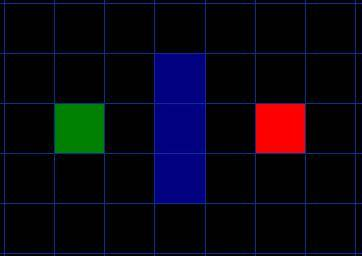
\includegraphics[width=0.4\textwidth]{aestrella/screen1.jpg}
  \caption{Escenario construido con mosaicos discretos. El problema de búsqueda de caminos consiste en encontrar una ruta desde el cuadro verde al cuadro rojo.}
  \label{fig:fig1P4}
\end{figure}

Si el mundo donde se encuentran nuestros personajes es continuo, el primer paso que debemos hacer es simplificar el área de búsqueda, dividiendo nuestro mundo en una rejilla de mosaicos cuadrados.  En los videojuegos algunos mundos ya son así desde un prinicipio.  En el caso de robótica se puede proceder a crear rejillas de ocupación discretizando las coordenadas del plano y representando al mundo con mosaicos ocupados/libres, semejantes a los de los videojuegos.  Con esto, podremos representar el mundo con una matriz bidimensional. Cada posición en la matriz representará un mosaico del mundo, el cual será transitable o no transitable. Entonces, el objetivo del algoritmo A* es calcular a qué mosaico nos debemos mover en cada turno para lograr llegar al punto B. Una vez calculado esto, el personaje del juego se moverá del centro del mosaico donde se encuentra actualmente al centro del mosaico obtenido con A*.  Observa entonces que cada mosaico del mundo es un estado posible para nuestro personaje.

A los puntos centrales dentro del mosaico se les llama \classname{nodos}. Pudimos haber dividido el mundo en círculos, en hexágonos o triángulos, cada mundo puede tener características diferentes y ser simplificado de distintas formas.  Nosotros usaremos cuadrados.

Ahora pensaremos en el mundo como un grafo.  Cuando dos mosaicos son adyacentes y es posible desplazarse de uno hacia el otro, decimos que hay un arista conectándolos.  De este modo, el algoritmo que busca la ruta más corta entre el punto A y el punto B es un recorrido sobre un grafo.

\subsection{Iniciando la b\'usqueda}

Después de haber simplificado el área de búsqueda en nodos, el siguiente paso es dirigir una búsqueda para encontrar el camino más corto. En el algoritmo A* lo hacemos empezando desde el punto A, comprobando los cuadros adyacentes (estados sucesores) y generalmente buscando hacia fuera hasta que encontremos nuestro destino.

\noindent Empezamos la búsqueda haciendo lo siguiente:

\begin{enumerate}
  \item Comenzamos en el punto inicial A y lo añadimos a una \textbf{lista abierta} de cuadrados a tener en cuenta. La lista contiene los cuadrados que podrían formar parte del camino que queremos tomar, pero que quizás no lo hagan. Básicamente, esta es una lista de los cuadrados que necesitan ser considerados. Si, por azares del destino, el punto A es igual al punto B, terminamos nuestra ejecución con un plan vacío: el personaje no necesita hacer nada, ya está en su destino.
  
  \item Sacamos el cuadro inicial A de la lista abierta y lo añadimos a una \textbf{lista cerrada} de cuadrados que no necesitan ser vistos de nuevo.
  
  \item Nos fijamos en todos los cuadrados alcanzables o transitables adyacentes al punto de inicio, ignorando cuadrados con muros, agua u otros terrenos prohibidos. Se añaden a la lista abierta también. Por cada uno de esos cuadrados, guardamos el punto A como su \textbf{cuadrado padre}. El cuadrado padre es muy importante para trazar nuestro camino.  La estructura dentro de la cual guardaremos esta información, y que ofreceremos a la lista abierta, se llama \textbf{nodo de búsqueda}.
\end{enumerate}

En este punto, se tendrá algo como la figura~\ref{fig:fig2P4}. En este diagrama, el cuadrado verde oscuro del centro es el cuadrado de inicio. Está bordeado de azul claro para indicar que el cuadrado ha sido añadido a la lista cerrada. Todos los cuadros adyacentes están ahora en la lista abierta para ser considerados. Cada uno tiene un puntero gris que señala a su padre, el cual es el cuadro inicial.

\begin{figure}[h]
  \centering
  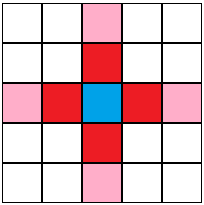
\includegraphics[width=0.3\textwidth]{aestrella/screen2.png}
  \caption{Mosaicos en la lista abierta con referencia a su padre.}
  \label{fig:fig2P4}
\end{figure}


Después, elegimos uno de los cuadrados adyacentes de la lista abierta y más o menos repetimos el proceso anterior. Pero, ¿qué cuadro se debe elegir? Aquel que tenga costo estimado \(f(n)\) más bajo.

\subsection{Puntuando el camino}

La clave para determinar qué cuadrados usaremos para resolver el camino está en la siguiente ecuación:\medskip

\begin{center}
\(f(n) = g(n) + h(n)\)
\end{center}\medskip

donde:

\begin{itemize}
  \item \(g(n)\) es el costo del movimiento para ir desde el punto inicial A a un cierto cuadro \(n\) de la rejilla, siguiendo el camino generado para llegar ahí.
  \item \(h(n)\) es el costo del movimiento estimado para ir desde ese cuadro \(n\) hasta el destino final, el punto B. Esto se conoce como la heurística. Aquí se verá una forma de calcular la heurística, pero no es la única.
\end{itemize}

Nuestro camino se genera al ir repetidamente a través de nuestra lista abierta eligiendo el cuadrado con la puntuación \(f(n)\) más baja. Este proceso se describirá con más detalle un poco más adelante. Primero veamos más de cerca cómo calculamos esta puntuación.

Tal y como está descrito arriba, \(g(n)\) es el costo del movimiento para ir desde el punto de inicio a un cuadro \(n\) usando el camino generado para llegar ahí. En esta práctica asignaremos un costo de 10 a cada cuadro vertical u horizontal hacia el que nos movamos, y un costo de 14 para un movimiento diagonal. Usamos estos números ya que es más simple poner 14 que \(\sqrt{2}\times10\) y porque usar números enteros es mucho más rápido para la computadora. Pronto descubrirás que los algoritmos de búsqueda pueden ser muy lentos si no usas atajos como éste.

Ahora que hemos calculado el costo \(g(n)\) mediante un camino específico hasta cierto cuadro, la forma de resolver el costo \(g(n)\) del cuadro vecino suyo es tomar el costo \(g(n)\) de su padre, y luego añadirle 10 o 14 dependiendo de si el movimiento para llegar a él es ortogonal o se realiza en diagonal con respecto al cuadro padre.

\(h(n)\) puede ser estimado de diferentes maneras. El método que usaremos aquí se llama el método Manhattan, donde se calcula el número total de cuadros movidos horizontalmente y verticalmente para alcanzar el cuadrado destino desde el cuadro actual, sin hacer uso de movimientos diagonales e ignorando cualquier obstáculo. Luego multiplicamos el total por 10. Se llama método Manhattan porque es como calcular el número de manzanas que hay desde un lugar a otro, donde no puedes acortar atravesando en diagonal una manzana. Es una estimación de la distancia que queda, no necesariamente coincide con la distancia real, es por eso que se llama heurística.

Observa que, mientras que \(g(n)\) solamente se puede calcular conforme se van eligiendo los nodos durante la búsqueda, el valor de \(h(n)\) sólo depende del punto B y el cuadrado \(n\), por lo que basta con calcular \(h(n)\) una sola vez y lo puedes hacer en cualquier momento.

\(f(n)\) se calcula sumando \(g(n)\) y \(h(n)\). El resultado del primer paso en nuestra búsqueda puede verse en la figura~\ref{fig:fig3P4}. Las puntuaciones \(f(n)\), \(g(n)\) y \(h(n)\) están escritas en cada cuadrado. En el cuadro inmediatamente a la derecha del cuadro inicial, se escribieron las letras F, G y H para indicar dónde se encuentran los valores de \(f(n)\), \(g(n)\) y \(h(n)\).

\begin{figure}[h!]
  \centering
  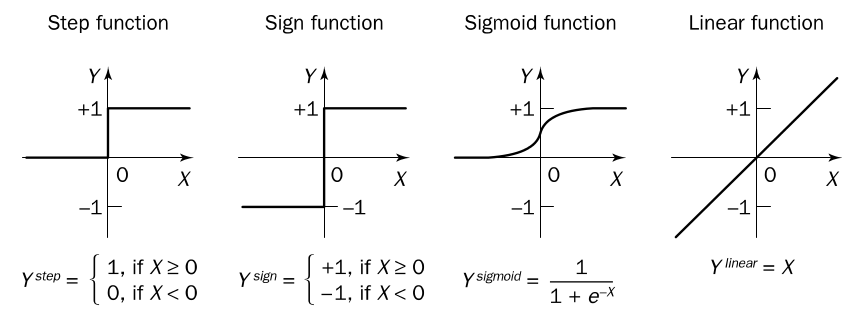
\includegraphics[width=0.5\textwidth]{aestrella/screen3.png}
  \caption{Cálculo de \(f\),\(g\) y \(h\) que se agregan a la lista abierta.}
  \label{fig:fig3P4}
\end{figure}

Así pues, observaremos algunos ejemplos de estos cuadros. En el cuadrado con letras, \(g(n)=10\). Esto es debido a que está solo a un cuadro del cuadrado inicial en dirección horizontal. Los cuadrados inmediatamente encima, abajo y a la izquierda del cuadrado inicial tienen todos el mismo valor \(g(n)\) de 10. Los cuadros diagonales tienen un valor \(g(n)\) de 14.

Las puntuaciones \(h(n)\) se calculan estimando la distancia Manhattan hasta el cuadrado rojo objetivo, moviéndose solo horizontal y verticalmente e \textbf{ignorando el muro} que está en el camino. Usando este método, el cuadro a la derecha del inicial, está a 3 cuadros del cuadrado rojo con una puntuación \(h(n)\) de 30. El cuadrado está a sólo 4 cuadros de distancia (recuerda que solo nos movemos en dirección horizontal y vertical) con una puntuación \(h(n)\) de 40. Probablemente podrás calcular las puntuaciones \(h(n)\) para los demás cuadros.  Observa que, para este mapa donde se permiten movimientos en diagonal, esta heurística no es admisible.

\subsection{Continuando la b\'usqueda}

Para continuar la búsqueda, simplemente elegimos la puntuación \(f(n)\) más baja de todos aquellos que estén en la lista abierta. Para que esta operación se realize lo más eficientemente posible, la lista abierta se implementará con una cola de prioridades. Después hacemos lo siguiente con el cuadro seleccionado:

\begin{enumerate}
  \item Lo sacamos de la lista abierta y lo añadimos a la lista cerrada.  

  \item Comprobamos todos los cuadrados adyacentes:
  
  \begin{enumerate}
   \item Ignorando aquellos que estén en la lista cerrada o que sean intransitables o a los que no se puede pasar: terrenos con muros, agua o cualquier terreno prohibido.
   
   \item Añadimos los cuadros a la lista abierta si no están ya en esa lista. Hacemos que el cuadro seleccionado sea el \textbf{padre} de los cuadros nuevos.
   
   \item Si el cuadro adyacente ya está en la lista abierta, comprobamos si el camino nuevo a ese cuadro es mejor que el que tenía, es decir, si el valor de \(g(n)\) con este padre es menor que el que se había estimado con su padre anterior. Si no es así, no haremos nada. Por otro lado, si el costo \(g(n)\) del nuevo camino es más bajo, cambiamos el padre del cuadro adyacente al cuadro seleccionado (en el diagrama superior, cambia la dirección del puntero para que señale al cuadro seleccionado). Finalmente, recalculamos \(f(n)\) y \(g(n)\) de ese cuadrado.
  \end{enumerate}
\end{enumerate}


\begin{figure}[h!]
  \centering
  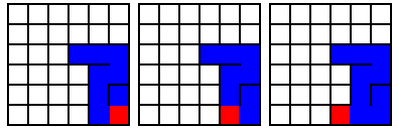
\includegraphics[width=0.95\textwidth]{aestrella/screen5.png}
  \caption{Ejecución completa del algoritmo.}
  \label{fig:fig4P4}
\end{figure}

La \fref{fig:fig4P4} muestra la ejecución completa del algoritmo para un escenario ligeramente más complejo.  En esta imagen también se muestra el contenido final de las estructuras auxiliares, las listas cerrada y abierta.


\section{Desarrollo e implementaci\'on}

Para esta práctica, considerate un miembro nuevo en un compañía de programación de videojuegos.  El resto del equipo ha estado trabajando en un \textit{remake} de Pacman con \code{JavaFX} y a ti te han asignado la siguiente tarea: programar al más férreo perseguidor de Pacman, el fantasma rojo \textbf{\textit{Sombra}}, mejor conocido como Blinky. Para ello, has decidido utilizar el mejor algoritmo para mundos finitos deterministas: A*.

Para realizar esta tarea se te entrega el código con el escenario listo para jugar y la documentación que han elaborado tus colegas.  El código aún no está terminado, pero ya incluye como muestra el primer nivel del juego y está listo para añadirle archivos de configuración con cualquier otro nivel.  Igualmente el código para controlar a Pacman usando las flechas del teclado ya funciona.  El único detalle es que Sombra aún no persigue a Pacman, se mueve siempre en una dirección fija que, lo notarás de inmediato, no lo lleva muy lejos.

El programa está compuesto por varios paquetes y clases pero como está diseñado con orientación a objetos, sólo necesitas entender algunas clases para agregar el algoritmo que necesita Sombra.  El diagrama UML de la \fref{fig:umlestrella} te muestra los paquetes, clases, atributos y métodos que son relevantes para tu tarea.

\begin{sidewaysfigure}
  \centering
  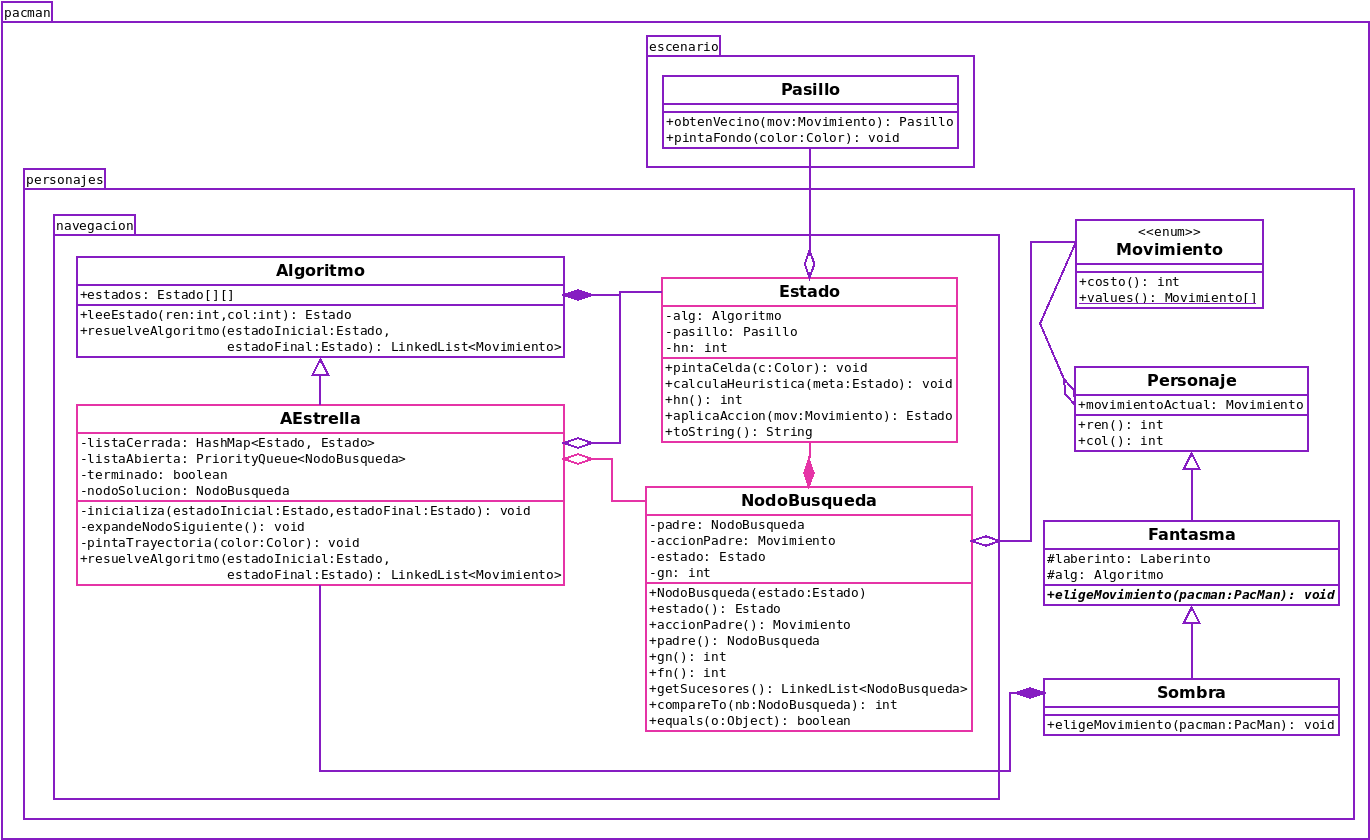
\includegraphics[width=\textwidth]{aestrella/UMLSombra.png}
  \caption{UML con las clases relevantes para programar el algoritmo de navegación para Sombra.  Las clases con métodos a implementar se muestran en rosa.}
  \label{fig:umlestrella}
\end{sidewaysfigure}

\subsection{Implementaci\'on}

Tu trabajo consiste en implementar la función:

\code{LinkedList<Movimiento> resuelveAlgoritmo(Estado estadoInicial, Estado estadoFinal)}

\noindent de la clase \code{pacman.personajes.navegacion.AEstrella}.
La variable \code{estadoInicial} contiene información con las coordenadas de la casilla inicial, mientras que \code{estadoFinal} indica a qué casilla se quiere ir.  El trabajo de esta función es devolver la secuencia de acciones que se deben realizar (movimientos) hasta llegar a la casilla final.

Para que ubiques mejor cómo será usada esta función te informan que, de momento, el estadoInicial corresponde a la posición actual de Sombra y estadoFinal es la posición de Pacman.  Sombra manda llamar esta función en cada tick del reloj con las nuevas posiciones suya y de Pacman.  De hecho, lo único que se utiliza es el primer movimiento de la trayectoria... pero no te confíes, las cosas pueden cambiar, otras optimizaciones podrían ser introducidas y por lo tanto debes calcular la lista completa de movimientos.  Aunque estos detalles son irrelevantes para tu código, saber cómo será usado te ayudará a visualizar lo que necesitas hacer.  Sin embargo, observa que por ser general, esta función podría llegar a utilizarse no sólo para mover a Sombra sino que, en algún momento, otro fantasma con otro comportamiento también podría aprovecharla.  Por ejemplo, el encargado de las emboscadas \textbf{\textit{Pinky}} podría usar A* para llegar a la esquina más cercana a Pacman enviado como parámetros sus coordenadas y las de dicha esquina.  Por lo tanto, no debes usar información de más o de menos confiándote en el estado actual de la aplicación, ni afectar el resto del juego con intervenciones innecesarias para que tu código sea reutilizable con facilidad.

Para ayudarte a realizar esta tarea el paquete te ofrece las herramientas siguientes:

\begin{enumerate}
 \item La clase \code{Estado} pertenece al subpaquete \code{navegación}.  Es una especie de envoltura con una referencia a un \code{Pasillo} por donde puede pasar el fantasma.  Un objeto de este tipo puede almacenar la información de ejecución relevante para el algoritmo A* como es el valor de la función \(h(n)\).  De este modo te brinda acceso al estado en el mundo (el laberinto donde se encuentran nuestros personajes) y te brinda un espacio para no afectar al mundo con información que sólo concierne al algoritmo de navegación de un fantasma.
 
 \item La superclase \code{Algoritmo} se encarga de inicializar, tras la creación del laberinto, un arreglo de objetos tipo \code{Estado}.  De este modo cuentas ya con un objeto estado por cada pasillo en el laberinto, en el mismo renglón y columna que el pasillo en el mundo.  Ojo, los valores de la heurística $h(n)$ cambian cada vez que cambia el lugar al quiere moverse el fantasma, así que recuerda recalcular tantos valores como sean necesarios cada vez que ejecutes el algoritmo con metas distintas.
 
 \item La clase \code{NodoBusqueda} contiene la información del grafo de búsqueda que va generando A* conforme explora los estados.  Por eso su primer atributo es una referencia al estado que está explorando.  También aquí se almacena el valor de $g(n)$, pues este valor depende de la ruta que se siga para llegar al estado $n$ desde el estado inicial; por ello mismo incluye la referencia al nodo padre y la acción que se realizó para llegar al estado que contiene.  Recuerda que, en general, varios nodos de búsqueda podrían apuntar al mismo estado.  Como en esta práctica se realizará una búsqueda en grafo no será el caso.
 
 \item La clase \code{Pasillo} ya representa, de hecho, la gráfica de estados por donde puede transitar un personaje, pues cada pasillo contiene referencias a sus pasillos vecinos.  Puedes acceder a ellos mediante el método \code{obtenVecino(Movimiento mov)}.  Te servirá para generar los estados sucesores de cada estado.
\end{enumerate}

Los métodos que deberás implementar son los siguientes:

\begin{enumerate}
 \item En la clase \code{Estado} la función:
 \begin{enumerate}
  \item \code{calculaHeuristica(Estado meta)}
 \end{enumerate}

 \item En la clase \code{NodoBusqueda}:
 \begin{enumerate}
  \item \code{LinkedList<NodoBusqueda> getSucesores()}
 \end{enumerate}


 \item En la clase \code{AEstrella}:
 \begin{enumerate}
  \item \code{LinkedList<Movimiento> resuelveAlgoritmo(Estado estadoInicial, Estado estadoFinal)}
 \end{enumerate}
 se te sugiere la implementación de dos métodos auxiliares:
 \begin{enumerate}
  \item \code{inicializa(Estado estadoInicial, Estado estadoFinal)}
  \item \code{void expandeNodoSiguiente()}
 \end{enumerate}
 Como son métodos privados, tienes la libertad de utilizarlos o modificarlos a tu gusto.  Se te provee con \code{pintaTrayectoria(Color color)} para ayudarte a depurar tu código.

\end{enumerate}

\section{Requisitos y resultados}

Los requisitos para tu trabajo son los siguientes:

\begin{enumerate}
 \item Para implementar el algoritmo puedes agregar atributos sólo si realmente necesitas recordar los valores de esas variables entre distintas llamadas a los métodos de la clase, únicamente en las clases marcadas con rosa.
 
 \item Es estas clases también puedes agregar métodos auxiliares si lo consideras necesario. De hacerlo, no olvides documentar cual es su función.
 
 \item No debes agregar ni atributos ni funciones a ninguna otra clase, ya tienes toda la información que necesitas; piensa que el resto del programa está siendo desarrollado por otros compañeros de la empresa y no tienes permiso de tocar sus componentes.
\end{enumerate}

Cuando termines tu implementación podrás ver a Sombra persiguiendo a Pacman por la ruta óptima; la única forma de alejarlo un poco será transportándose por los pasillos que sacan a Pacman por un lado de la pantalla y lo regresan por el otro.  Si gustas, borrar e iluminar la ruta que sigue Sombra a cada paso es muy fácil ya teniendo la trayectoria completa.

\begin{figure}
  \centering
  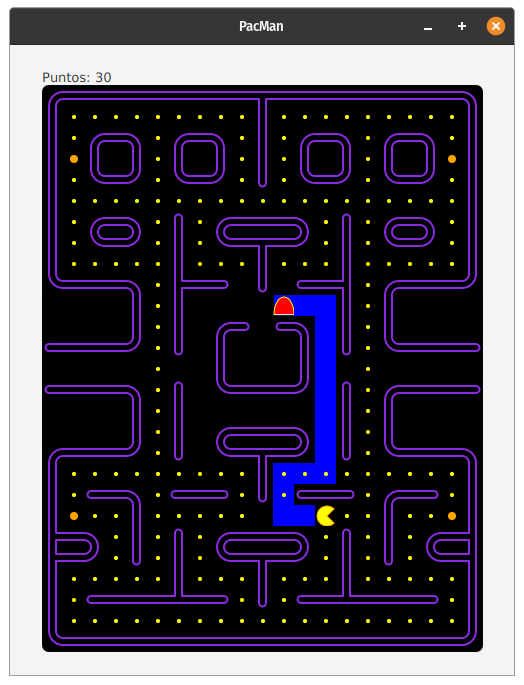
\includegraphics[width=0.4\textwidth]{aestrella/screen6.png}
  \caption{Sombra persiguiendo a Pacman por la ruta óptima.}
  \label{fig:fig1P4}
\end{figure}
